

\documentclass[a4paper,twoside]{article}

\usepackage{epsfig}
\usepackage{subfigure}
\usepackage{calc}
\usepackage{amssymb}
\usepackage{amstext}
\usepackage{amsmath}
\usepackage{amsthm}
\usepackage{multicol}
\usepackage{pslatex}
\usepackage{apalike}
\usepackage{SCITEPRESS}     % Please add other packages that you may need BEFORE the SCITEPRESS.sty package.

\usepackage{tikz}
\usepackage[utf8]{inputenc}
\usetikzlibrary{mindmap}
\usepackage[hidelinks,pdfencoding=auto]{hyperref}
\usepackage{dirtree}

\subfigtopskip=0pt
\subfigcapskip=0pt
\subfigbottomskip=0pt

\begin{document}

\title{Data Format for Storing ANT+ Sensors Data}

\author{\authorname{Petr Je\v{z}ek\sup{1}, Roman Mou\v{c}ek\sup{1}}
\affiliation{\sup{1}Department of Computer Science and Engineering, New Technologies for the Information Society, Faculty of Applied Sciences, University of West Bohemia, Plzen, Czech Republic}
\affiliation{}
\email{\{jezekp, moucek\}@kiv.zcu.cz}
}

\keywords{ANT+, NIX, sensor, data/metadata storage, EEGBase, data format, eHealth.}

\abstract{Medical treatment of sudden and especially chronic diseases has become more expensive. People suffering from a variety of diseases had been traditionally treated in hospitals for a~long time. Fortunately, the current situation has been changing also thanks to relatively cheap body sensors and development of systems for home treatment. It brings inconsiderable cost savings and improves patients' comfort. On the other hand, it puts demands on the used technical infrastructure and home treatment system developers who must solve integration of different systems. A~crucial point is a~definition of unified data formats facilitating transfer and storage of data to/in remote databases. There are standards and APIs such as Zigbee, Bluetooth low energy or ANT+ that define a protocol for data transfer. However, they do not define a~suitable format for long term data storing. In this paper, data coming from ANT+ sensors have been studied and metadata related to all kinds of body sensors and raw data and metadata specific to individual sensors have been defined. Then a~framework organizing data and metadata obtained from ANT+ sensors into an open and general data format suitable for long term storage of sensor data is introduced. Finally, a~sample use-case showing the transfer of data from a~sensor into a~data storage is presented.}

\onecolumn \maketitle \normalsize \vfill


\section{Introduction}\label{sec:intro}
Medical treatment of sudden and especially chronic diseases has become more expensive, especially with aging population. For instance, there were around 23 million people in the world affected with heart failure in 2011 \cite{bui2011epidemiology}. These people had been usually treated in hospitals for a~long time. The situation has been changing at present because relatively cheap solutions for home treatment have appeared in the market~\cite{4761985},	 \cite{5333913} and patients can be moved from hospitals to their homes sooner. It brings advantages of a~better comfort for patients and makes treatment generally cheaper.

Home treatment systems use a set of wearable sensors, usually powered from batteries, for monitoring of health or fitness level. They have to operate for a~long time period without possibility to change batteries frequently. That is why new protocols with low energy consumption such as ZigBee~\cite{Farahani:2008:ZWN:1457417}, Bluetooth Low Energy~\cite{heydon2012bluetooth} or ANT~\cite{zaloker2014ant} have been developed. Data from these sensors are transferred to remote servers where they are processed and visualized. Body Area Network (BAN) is an integration of sensors providing a~large data collection of body parameters.  When the number of sensors connected to BAN increases, requirements for the management, long term storage and sustainability of acquired data also increases.

Although there are some low energy consumption standards for data transfer, these are too fragmented to allow easy manipulation with obtained data. Of course, these standards also do not provide means for long term storage and management of transferred data. As a solution this paper presents how to use a~general data format called NIX~\cite{Stoewer:2014} for encapsulating and storing ANT+ sensor data.

The paper is organized as follows. Section~\ref{sec:state-of-the-art} deals with sensor infrastructure and description of data obtained from sensors. Section~\ref{sec:ant-plus-profiles} describes existing ANT+ profiles; the most suitable profiles for eHealth domain are selected. Section~\ref{sec:framework} introduces a~framework that facilitates conversion of sensor data to the NIX format. Section~\ref{sec:use-case} presents the usage of proposed transformation, a~simple use-case is provided. Section~\ref{sec:future-work} summarizes the work and provides an outlook to the future.

\section{State of The Art}\label{sec:state-of-the-art}

There are several approaches aiming to manage Body Area Networks data. These solutions use semantic web technologies or cloud infrastructures. Three layers ontology describing data from different sensors is presented in~\cite{mehmood2014ontology}. This ontology facilitates development of tools used for processing of sensor data. A~Sensor-Cloud infrastructure~\cite{5635688} represents physical sensors as virtual sensors stored in a~cloud infrastructure. Semantic Sensor Web \cite{4557983} is based on annotation of sensors data by means of Semantic Web. Such annotated data can be distributed on the Internet.


\section{ANT+ Profiles Discussion}\label{sec:ant-plus-profiles}
The ANT protocol is popular because of its low energy consumption and existence of suitable means for description of body parameters. 'Device profiles' (called ANT+) define data over the network in a consistent way~\cite{innovations2013ant} and facilitate development of sensors and management of sensor data in application programs.

ANT+ profiles support a large scale of activities such as cycling, walking, or measurement of body parameters such as heart rate, blood pressure, weight, or muscle oxygen. When browsing individual profiles in a detail we find the attributes that are common for all profiles, for example a device name, device status, manufacturer, signal strength or battery status. Then, there are attributes varying for individual profiles. Individual profile attributes represent raw sensor data or domain specific metadata while common attributes describe general metadata (see Figure~\ref{AntPlus}).


\begin{figure*}
\centering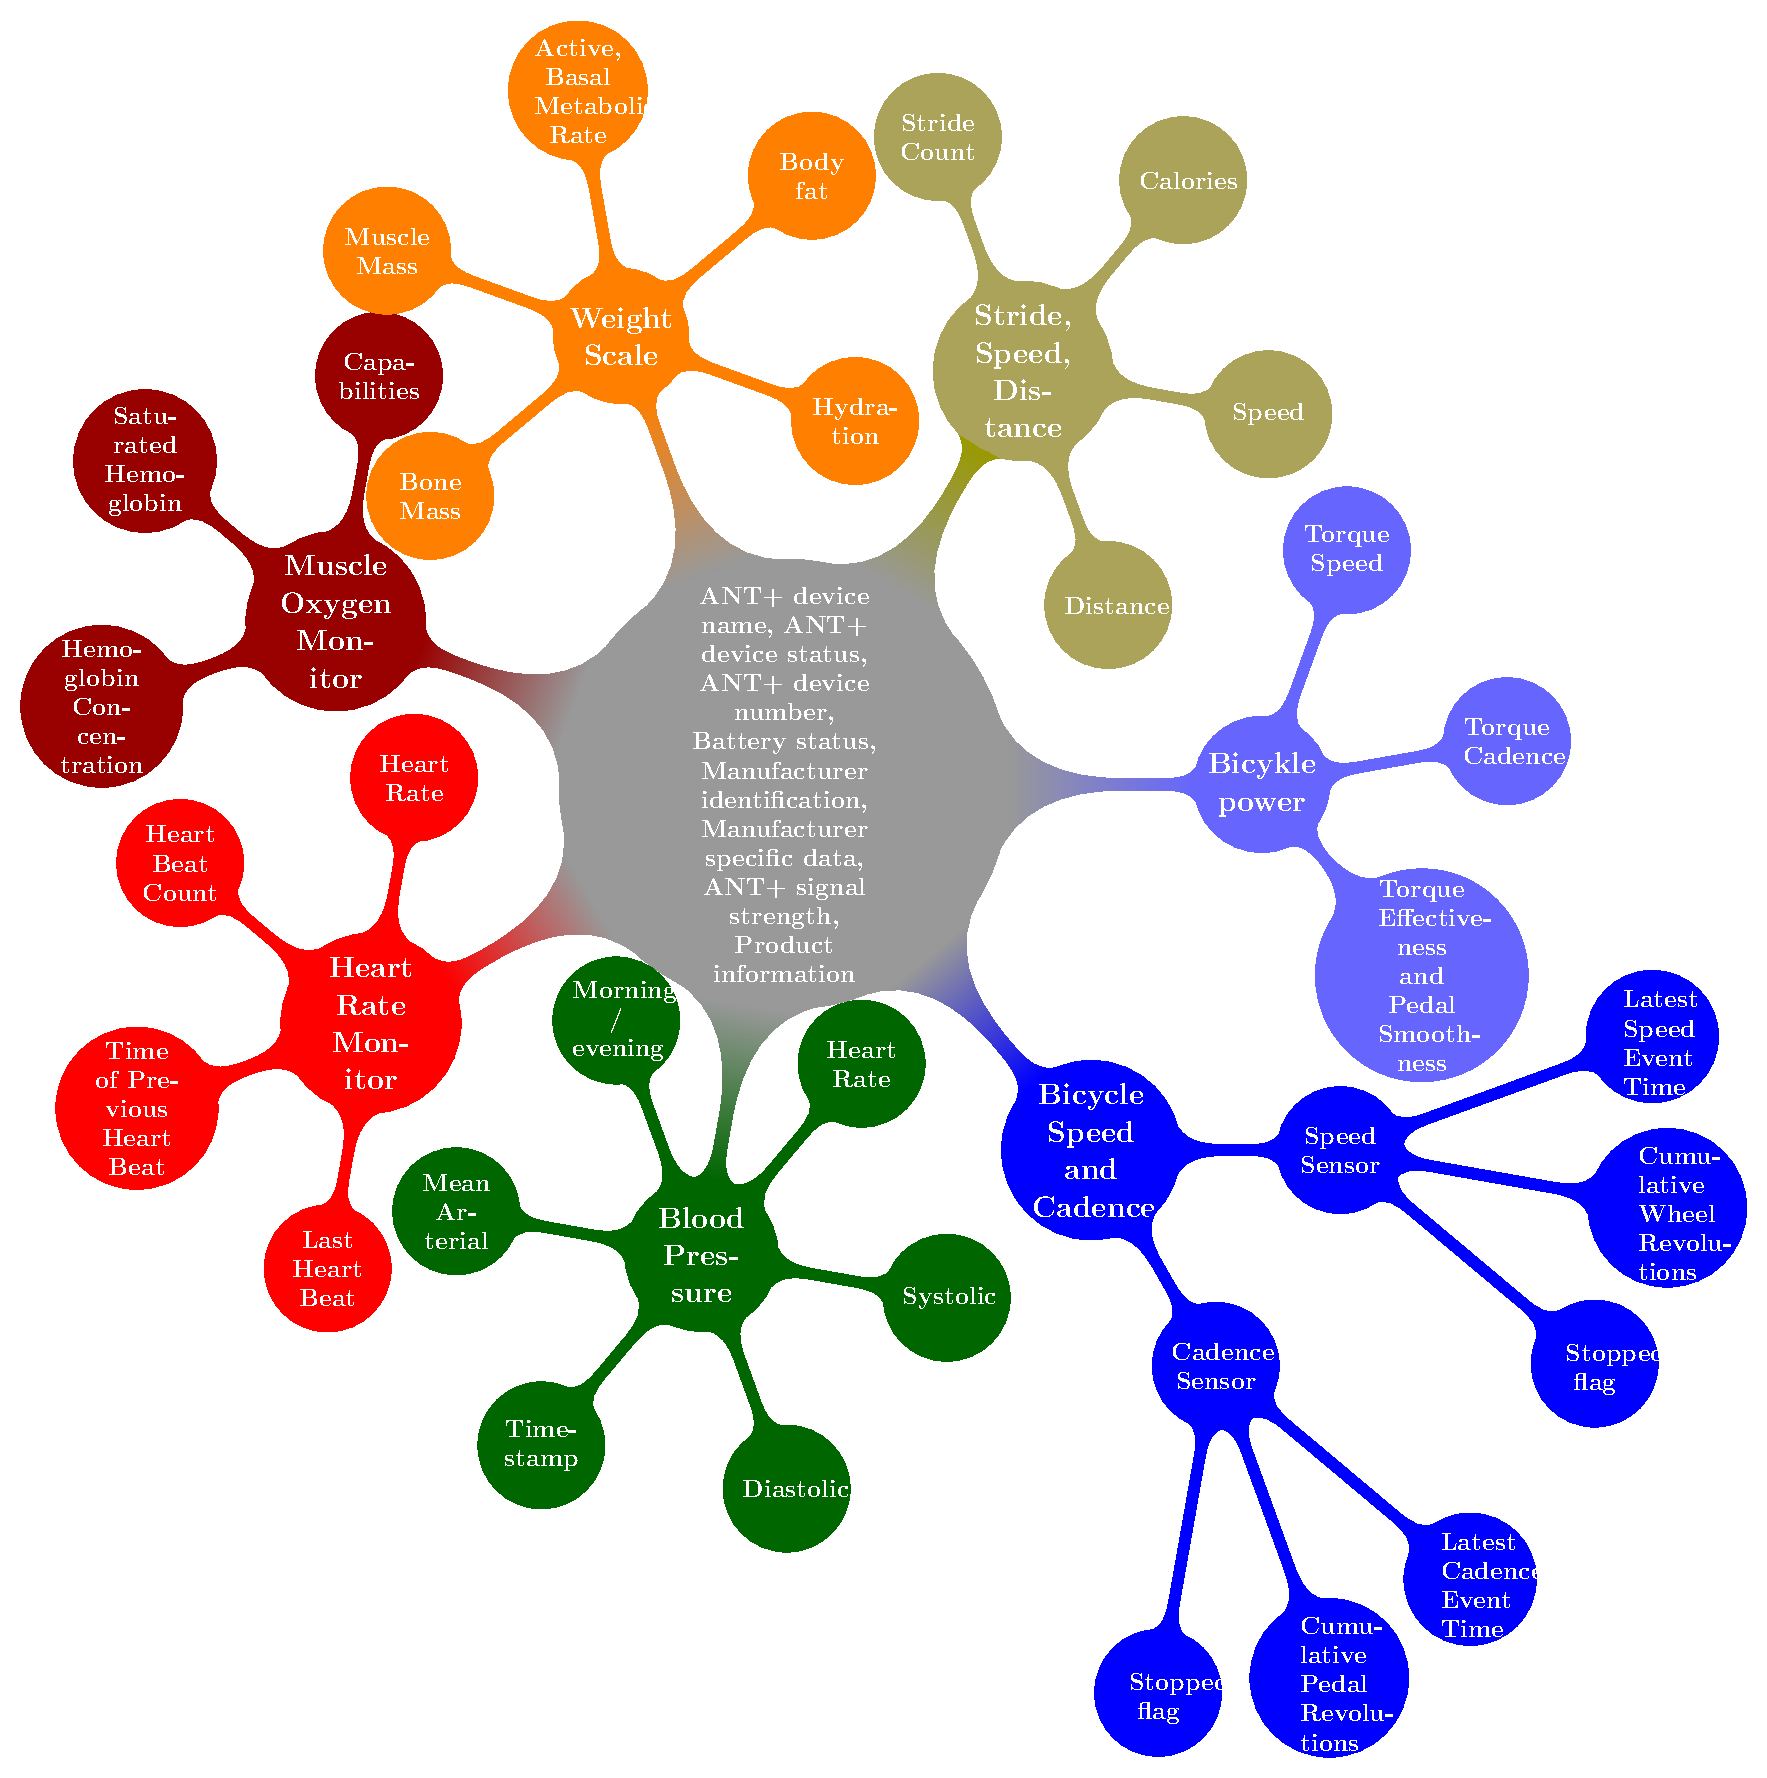
\includegraphics[width=14cm, height=10.5cm]{AntPlusProfiles}
\caption{\label{AntPlus}ANT+ Profiles Network}
\end{figure*}


\section{Proposed Framework}\label{sec:framework}

\subsection{Prerequisites}\label{sec:requirements}

Due to the absence of a suitable format/data structure for sensor data representation we have designed a framework for collection and storage of sensor raw data and metadata in a~defined structure. The used data structure/format has to be robust, flexible and widely accepted by scientific community to cover a~heterogeneous nature of sensor data, provide a long term data sustainability, and ensure its re-usability in third-party systems.

\subsection{Format Discussion}

Within a working group of International Neuroinformatics Coordinating Facility (INCF)~\cite{wvangeit:Bjaalie:JNeurosci:2007} and its Task Force on Electrophysiology\footnote{http://www.incf.org/programs/datasharing/ electrophysiology-task-force} there were introduced two approaches towards defining a~standard on electrophysiology data. The first one uses the Hierarchical Data Format (HDF5)~\cite{hdf5}. HDF5 is portable and extensible format supporting an unlimited variety of datatypes that is designed for flexible and efficient I/O operations with high volume and complex data. The second approach uses odML~\cite{10.3389/fninf.2011.00016} as a~free form tree-like structure of sections, properties and values suitable for metadata description. This simple, platform-independent and human-readable format also ensures compatibility with other systems developed within the community such as~\cite{10.3389/conf.fninf.2014.18.00029},~\cite{10.3389/conf.fninf.2014.18.00053},~and~\cite{10.3389/conf.fninf.2013.09.00025}. The next step of the task force, merging of these two approaches~\cite{10.3389/conf.fninf.2013.09.00069}, resulted in the proposal of the NIX format~\cite{Stoewer:2014} that provides a~data model for storing experimental data in HDF5 together with its metadata internally organized in the odML format. The NIX format is currently used in Helmholtz~\cite{10.3389/conf.fninf.2013.09.00025} and EEGBase~\cite{ISI:000306821100004} projects.

Although the NIX format was intended to be used in electrophysiology, its general definition makes it suitable for any time series data.


\subsection{Proposed Mapping}

We selected ANT+ profiles relating to person health and/or fitness level. Figure~\ref{AntPlus} shows common metadata (see the central circle) and domain specific raw data and metadata (see other circles). The NIX model consists of several main elements: Block, DataArray, Tag, MultiTag, Source, Group, and Dimension. Each element includes a~set of attributes (such as id, name, specific attributes) and link to metadata organized in the odML structure. We used a~simplified NIX model for mapping ANT+ elements. The Source element represents an ANT+ device, DataArray represents raw data, Dimension represents description of graph axes, and Block wraps a~complete record.


\section{Use Case}\label{sec:use-case}

The presented framework serves mainly to designers and programmers of the systems for home monitoring. Let's assume the following use-case. A programmer wants to implement a system for heart rate monitoring of elderly people. There are the following system requirements: sensors have to be easy to use and  sensors data must be easily transferred to a computer where they are stored and evaluated. Moreover, during regular medical checks a~physician uses long term records to check health condition of the patient and eventually starts a treatment. It means that both the patient and physician have access to the infrastructure that ensures data storing and management as well as data security, consistency and sustainability.

In this use-case we used the Garmin Premium Strap Heart Rate Monitor as a representative of ANT+ supporting devices. The Android SDK\footnote{http://developer.android.com/sdk/} was used to read ANT+ data into Android smart phones. We integrated this SDK into a custom mobile application MoBio\footnote{https://github.com/NEUROINFORMATICS-GROUP-FAV-KIV-ZCU/MoBio} that reads data from ANT+ sensors and store them on a~SD card. The user of MoBio can pair available sensors, record data and visualize them. This solution is available to a large number of users due to the existence of cheap Android smart phones and heart rate monitor straps on the market.

\begin{figure}

\dirtree{%
.1 Section.
.2 name = heart\_rate.
.2 type = metadata.
.2 Properties.
.3 Device name = Strap heart rate monitor.
.3 Device number = 1.
.3 Product Information = Garmin Premium Strap Heart Rate Monitor.
}
\caption{\label{odML}Metadata from the heart rate sensor in odML structure}
\end{figure}


\begin{figure*}
\centering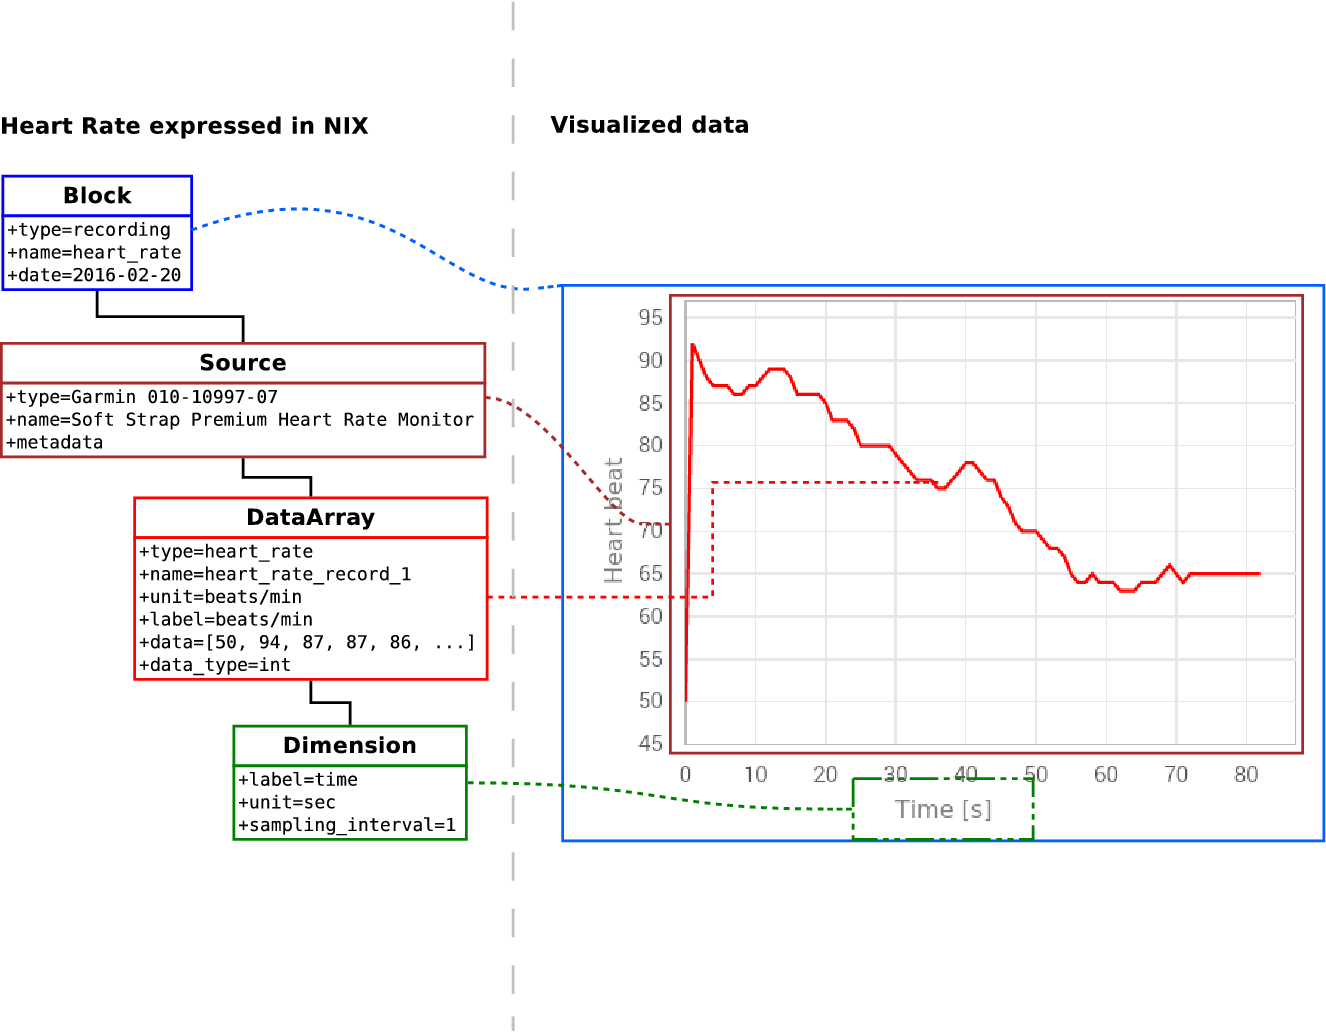
\includegraphics[width=11cm]{NIX-example.png}
\caption{\label{NIX-ex}Heart rate record in the NIX format}
\end{figure*}


Since our framework was also integrated into MoBio, recorded data can be stored in the NIX format. MoBio parses the record, metadata are transferred into a~structure with one section and several properties (see an example in Figure~\ref{odML}) and continuously read heart beats data are stored into the DataArray element (see an example in Figure~\ref{NIX-ex}). The Source element has an attribute metadata that contains a~link to the odML structure.




Once the data and metadata are stored they can be transferred to a suitable database. Figure~\ref{fig:EEGBase} shows the metadata stored and visualized in EEGBase. A~complete description of the experiment contains metadata from the Heart Rate strap. The raw data are stored as well.

\begin{figure}
  %\vspace{-0.2cm}
  \centering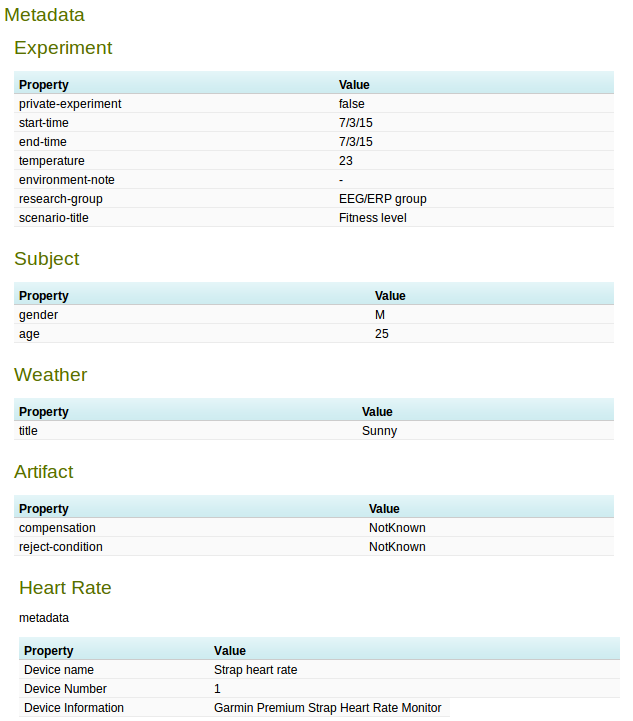
\includegraphics[width=8cm]{portal_example.png}
  \caption{Metadata stored in EEGBase}
  \label{fig:EEGBase}
 \end{figure}


\section{Conclusions and Future Work}\label{sec:future-work}

Together with raising popularity of sensors for home treatment several low energy standards have been defined. These standards enable data to be transferred from body sensors into common computers where they are processed and visualized. ANT+ supported by significant sensors producers is one of the most used standards. Although transfer protocols and several APIs for working with sensors are defined, an open standard for storing sensors data are not substantially provided. Since home treatment systems use proprietary data formats, they cannot be easily integrated with variety of sensors.

In this paper we overcome these difficulties by designing a~framework that maps data from ANT+ sensors into the open and generally applicable NIX format. The format brings advantages of two layers structure, metadata are structured using the flexible odML format and data are organized using the HDF5 format. Two layered organization of ANT+ sensors data is also a~significant contribution of this work.

The functionality of the framework is shown on a~simple use case. Within our future work the testing of a~large collection of sensors followed by data transfer to a few databases is supposed. We also plan to invite developers of home treatment systems to integrate the framework into their solutions. When the framework is fully tested, we start to work on the transformation of data using the Bluetooth low energy standard into the NIX format as well.


\section*{\uppercase{Acknowledgements}}

\noindent This publication was supported by the project LO1506 of the Czech Ministry of Education, Youth and Sports.

\bibliographystyle{apalike}
{\small
\bibliography{EMBC-2016,citations-ic4awe-2016,bibliography,neuroportals}}

\vfill
\end{document}

